\lecture{Sistemi di Stoccaggio Tradizionali}{26~-~01~-~2026}
%
%
\section{Layout di Magazzino}
Il magazzino non è solo un luogo di deposito, ma un nodo cruciale per la funzionalità aziendale, il cui peso economico e spaziale è significativo. Gli scopi principali sono la costituzione di una riserva di materiali, la loro conservazione e una disposizione razionale.
%
\paragraph{Flussi e Aree Funzionali} Le attività principali seguono un flusso logico: \\
Ricevimento (scarico, controlli) $\rightarrow$ Stoccaggio $\rightarrow$ Allestimento Ordini (picking, packaging) $\rightarrow$ Spedizione. \\
Esistono diverse configurazioni di layout per ottimizzare i flussi:
\begin{itemize}
    \item \textbf{Layout a U}: Ingresso e uscita sono sullo stesso lato. Vedi figura \ref{fig:layout_u}.
    \item \textbf{Layout a V}: Riduce le distanze percorse del 10\% ma richiede brusche sterzate. Vedi figura \ref{fig:layout_v}.
    \item \textbf{Layout Fishbone (a spina di pesce)}: Permette percorsi quasi rettilinei e riduce distanze/tempi del 23,5\%, ma richiede maggior spazio. Vedi figura \ref{fig:layout_fishbone}.
\end{itemize}
\begin{figure}
    \centering
    \begin{subfigure}{0.45\linewidth}
        \centering
        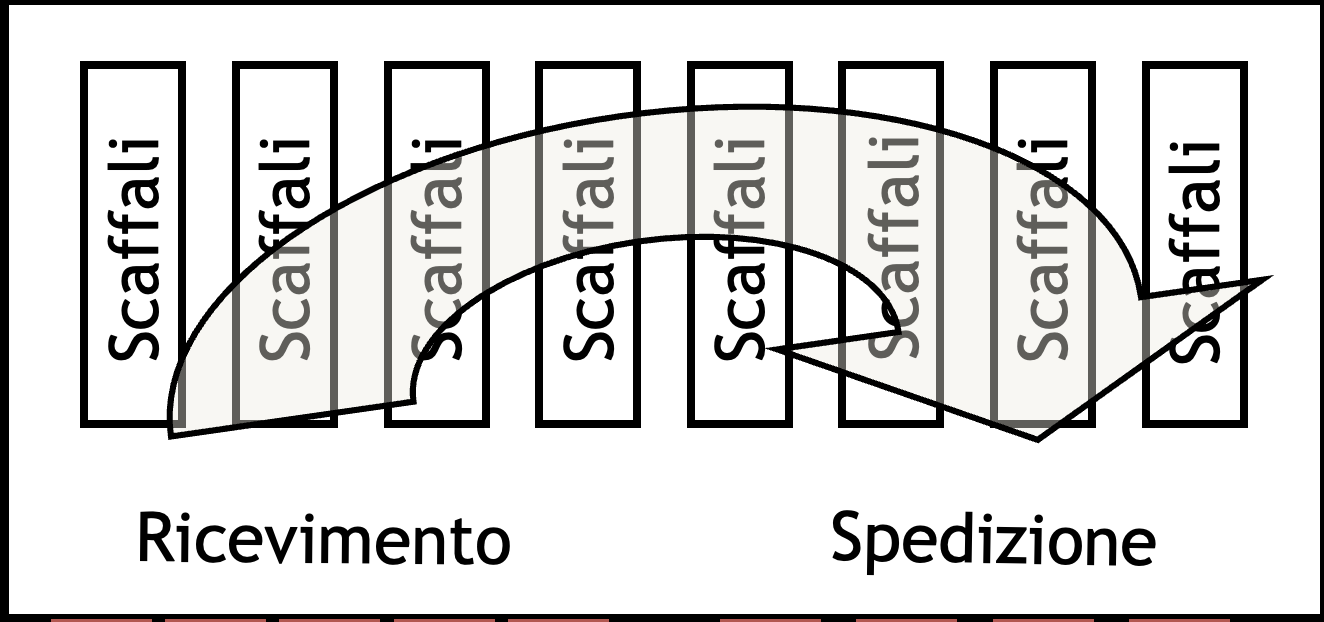
\includegraphics[width=\linewidth]{assets/Screenshot 2026-01-26 at 11.23.13.png}
        \caption{Layout a U}\label{fig:layout_u}
    \end{subfigure}
    \begin{subfigure}{0.45\linewidth}
        \centering
        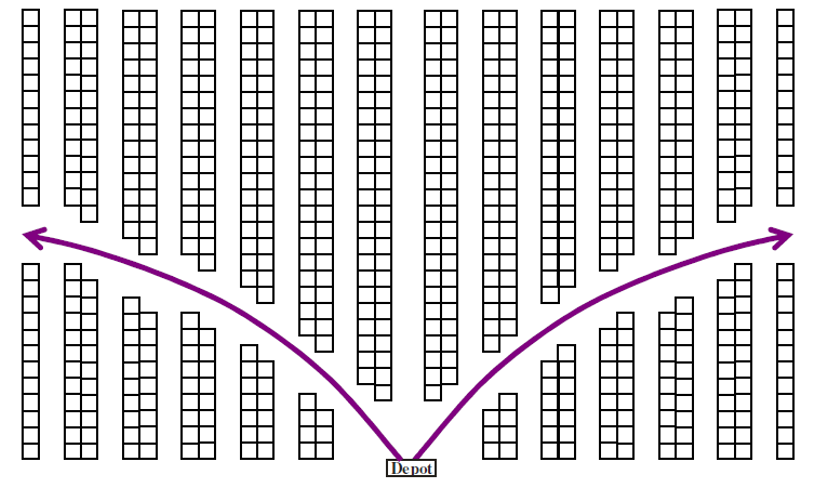
\includegraphics[width=\linewidth]{assets/21.png}
        \caption{Layout a V}\label{fig:layout_v}
    \end{subfigure}
    \begin{subfigure}{0.45\linewidth}
        \centering
        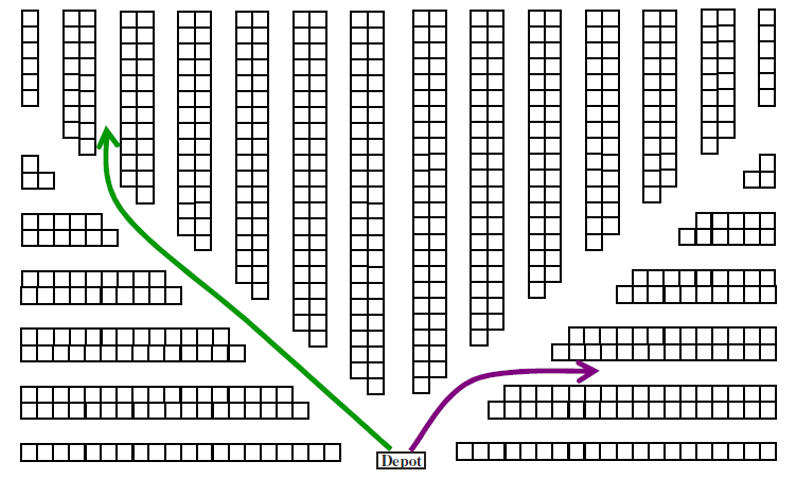
\includegraphics[width=\linewidth]{assets/22.png}
        \caption{Layout Fishbone}\label{fig:layout_fishbone}
    \end{subfigure}
    \caption{Layouts di Magazzino}\label{fig:layouts}
\end{figure}
%
\paragraph{Distanziamento Sociale} È fondamentale garantire una netta separazione tra le zone di contatto con l'esterno (ricevimento/spedizione) e le aree interne per evitare incroci di personale, utile anche per il distanziamento sociale. Se possibile, gestire il personale a turni separati e congelati, senza possibilità di cambio dei turni.

%
\subsection{Indici di Prestazione (KPI)}
Gli indici di prestazione (KPI) sono metriche utilizzate per valutare l'efficienza e l'efficacia delle operazioni di magazzino. Vedi tabella \ref{tab:kpi_summary} per un riepilogo.
%
\paragraph{Ricettività} La ricettività $ R $ è il numero massimo di Unità di Carico (UdC) stoccabili.
%
\paragraph{Selettività} La selettività $ I_{s} $ indica l'accessibilità diretta alle UdC.
\[
    I_{s} = \frac{\text{Numero di Codici Direttamente Accessibili}}{\text{Numero di Codici Totali}}
\]
Questo significa che se è presente un solo codice a magazzino, allora:
\[
    I_{s} = \text{Numero di Codici Direttamente Accessibili}
\]
Il risultato è una percentuale [$ \% $].

%
\paragraph{Coefficiente di Utilizzazione Superficiale}
\[
    C_{s} = \frac{S_{\text{stoccaggio}}}{S}
\]
Dove $ S_{\text{stoccaggio}} $ è la superficie del magazzino occupata dalle UdC ($ \si{m^2} $) e $ S $ è la superficie totale dell'area di stoccaggio ($ \si{m^2} $). Il risultato è una percentuale [$ \% $].

%
\paragraph{Coefficiente di Utilizzazione Volumetrico}
\[
    C_{v} = \frac{V_{\text{stoccaggio}}}{V}
\]
Dove $ V_{\text{stoccaggio}} $ è il volume del magazzino occupato dalle UdC ($ \si{m^3} $) e $ V $ è il volume totale dell'area di stoccaggio ($ \si{m^3} $). Il risultato è una percentuale [$ \% $].
%
\paragraph{Potenzialità di movimentazione}
Numero di UdC movimentabili nell'unità di tempo.
\[
    PM
\]
Il risultato è $ \si{UdC\per ora} $.

%
\paragraph{Giacenza Media} Calcolata come media ponderata delle quantità nel tempo:
\[
    G_{\text{media}} = \frac{q_{1}t_{1}+q_{2}t_{2}+\dots+q_{n}t_{n}}{t_{1}+t_{2}+\dots+t_{n}}
\]
Vedi figura \ref{fig:giacenza_media}.
\begin{figure}
    \centering
    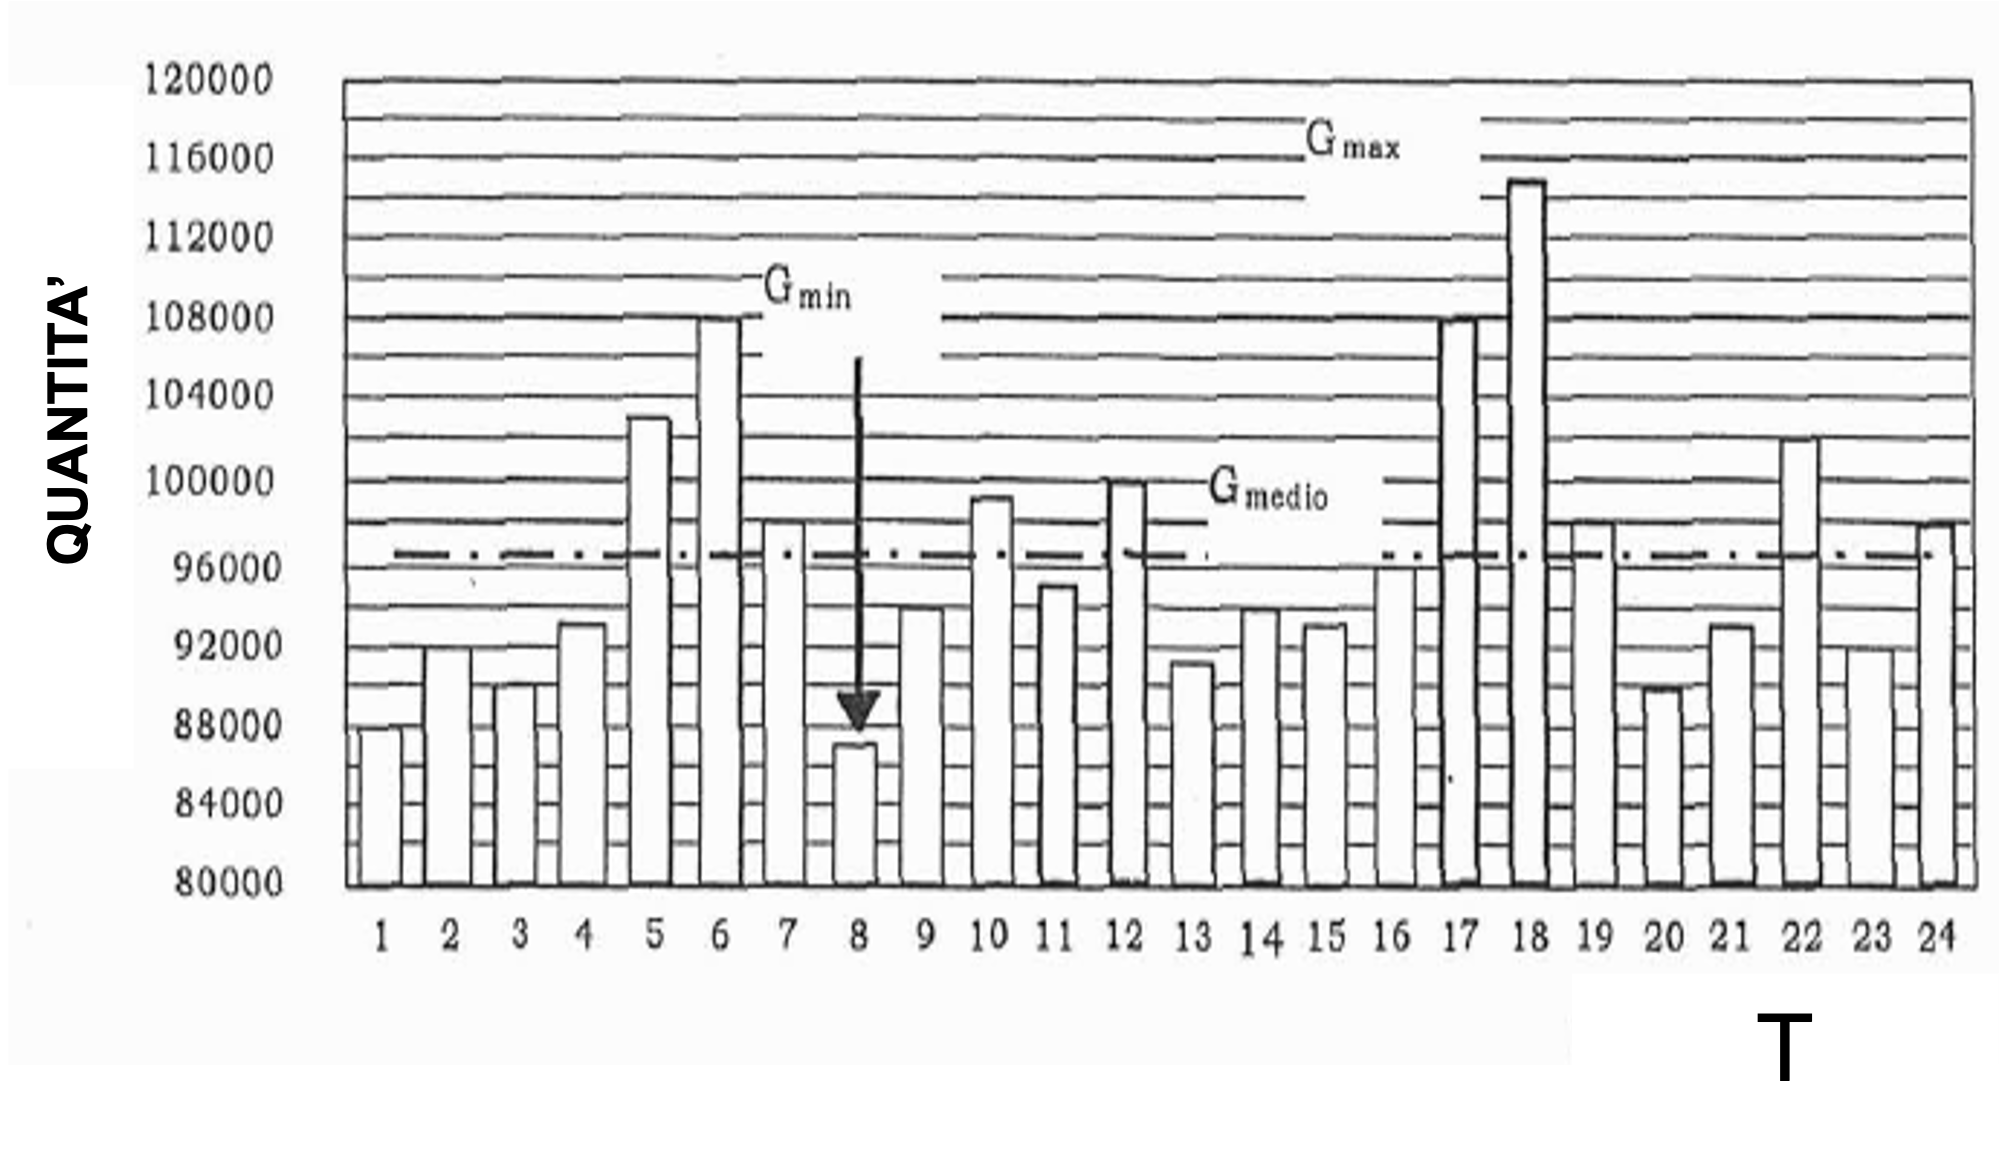
\includegraphics[width=0.5\linewidth]{assets/23.png}
    \caption{Giacenza Media}\label{fig:giacenza_media}
\end{figure}

%
\paragraph{Indice di Rotazione delle Merci}
\[
    I_{R} = \frac{U_{\text{transito}}}{G}
\]
Dove $ U_{\text{transito}} $ sono le uscite nel periodo T ($ \si{m^3}, \si{UdC} $, \dots) e $ G $ la giacenza media nel periodo T.
%
\subparagraph{Indice di Durata}
\[
    I_{D}=\frac{1}{I_{R}}
\]
%
\subparagraph{Giorni di Copertura}
\[
    GC = \frac{GG}{I_{R}}
\]
Dove $ GG $ sono i giorni lavorativi nel periodo T.
%
\paragraph{Indice di Honeycombing} Rapporto tra ubicazioni vuote e totali:
\[
    I_{H} = \frac{\text{Ubicazioni Vuote}}{\text{Ubicazioni Totali}}
\]

\begin{table}
    \centering
    \renewcommand{\arraystretch}{1.8} % Aumenta lo spazio verticale per le frazioni
    \begin{tabular}{llr} %
        \toprule
        \textbf{Indice}           & \textbf{Formula}                                                      & \textbf{Unità}     \\
        \midrule
        Ricettività               & $R$                                                                   & UdC                \\
        Selettività               & $I_{s} = \frac{\text{Codici Dir. Accessibili}}{\text{Codici Totali}}$ & \%                 \\
        Coeff. Util. Superficiale & $C_{s} = \frac{S_{\text{stoccaggio}}}{S}$                             & \%                 \\
        Coeff. Util. Volumetrico  & $C_{v} = \frac{V_{\text{stoccaggio}}}{V}$                             & \%                 \\
        Potenzialità di mov.      & $PM$                                                                  & \si{UdC\per ora}   \\
        Giacenza Media            & $G_{\text{media}} = \frac{\sum q_{i}t_{i}}{\sum t_{i}}$               & \si{m^3}, \si{UdC} \\
        Indice di Rotazione       & $I_{R} = \frac{U_{\text{transito}}}{G}$                               & -                  \\
        Indice di Durata          & $I_{D}=\frac{1}{I_{R}}$                                               & Periodo T          \\
        Giorni di Copertura       & $GC = \frac{GG}{I_{R}}$                                               & Giorni             \\
        Indice di Honeycombing    & $I_{H} = \frac{\text{Ubicazioni Vuote}}{\text{Ubicazioni Totali}}$    & \%                 \\
        \bottomrule
    \end{tabular}
    \caption{Riepilogo Indici di Prestazione (KPI) di Magazzino}\label{tab:kpi_summary}
\end{table}

%
\section{Warehouse Management System}
La gestione operativa è supportata dal WMS (Warehouse Management System), un software che pianifica, controlla e ottimizza i processi, offrendo visibilità sull'inventario e coordinando le attività fino alla spedizione.

È molto importante esaminare in modo analitico quali sono gli articoli sui quali esercitare un maggiore controllo. In tal caso si utilizza l'Analisi di Pareto (ABC), basata sui consumi annui o valore immobilizzato:
\begin{itemize}
    \item \textbf{Materiali di Classe A}: Pochi articoli (10-15\%) che valgono la maggior parte del valore (70-80\%).
    \item \textbf{Materiali di Classe C}: Molti articoli che valgono poco (5-10\% del valore).
    \item \textbf{Materiali di Classe B}: A seconda dei casi vengono associati alla classe A oppure C.
\end{itemize}
%
\section{Sistemi di stoccaggio}
I magazzini si dividono in \emph{Statici} (posizione UdC fissa) e \emph{Dinamici} (posizione variabile). Un'altra distinzione fondamentale è tra sistemi ``Operatore verso materiali'' (l'uomo va allo scaffale) e ``Materiali verso operatore'' (automazione).
%
\subsection{Magazzini Statici}
\begin{figure}
    \centering
    \begin{subfigure}{0.3\linewidth}
        \centering
        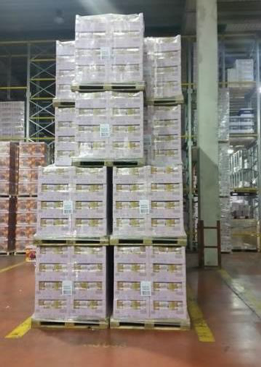
\includegraphics[width=\linewidth]{assets/24.png}
        \caption{Catasta}\label{fig:catasta}
    \end{subfigure}
    \begin{subfigure}{0.34\linewidth}
        \centering
        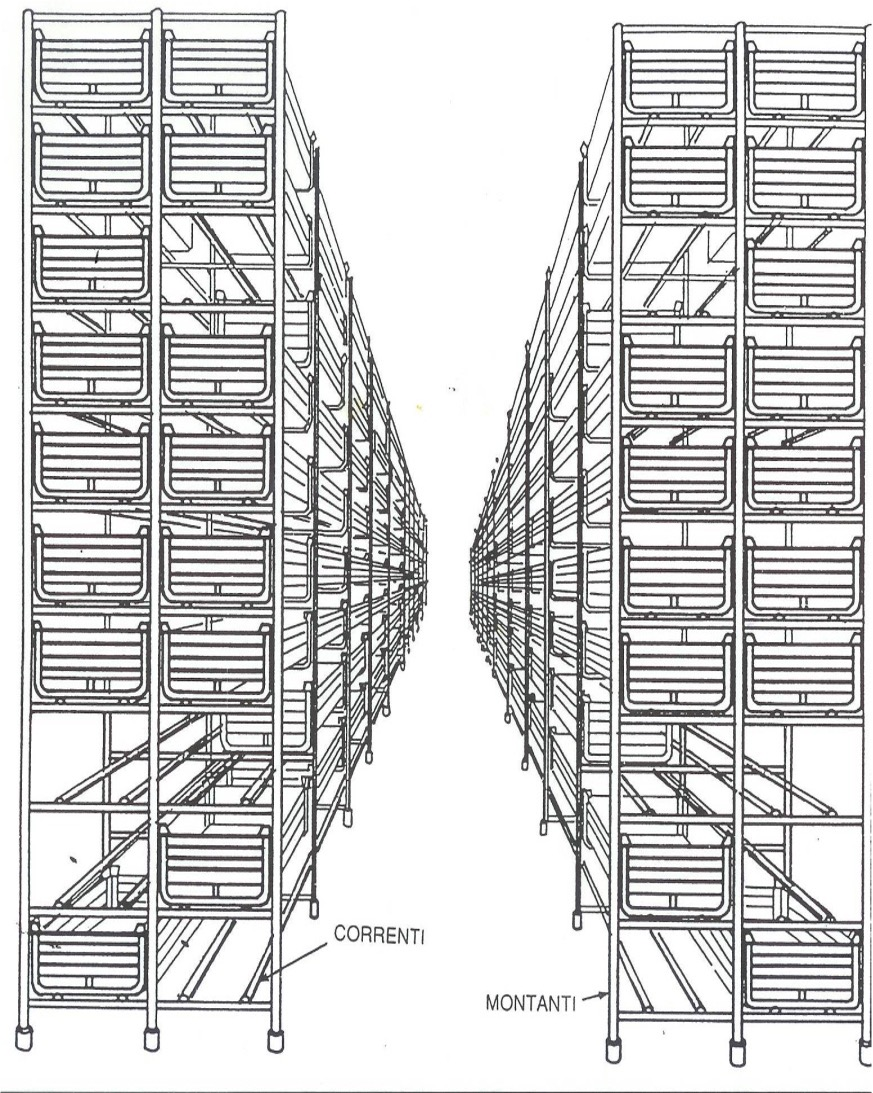
\includegraphics[width=\linewidth]{assets/25.jpg}
        \caption{Scaffalatura Tradizionale}\label{fig:scaffalatura_trad}
    \end{subfigure}
    \begin{subfigure}{0.5\linewidth}
        \centering
        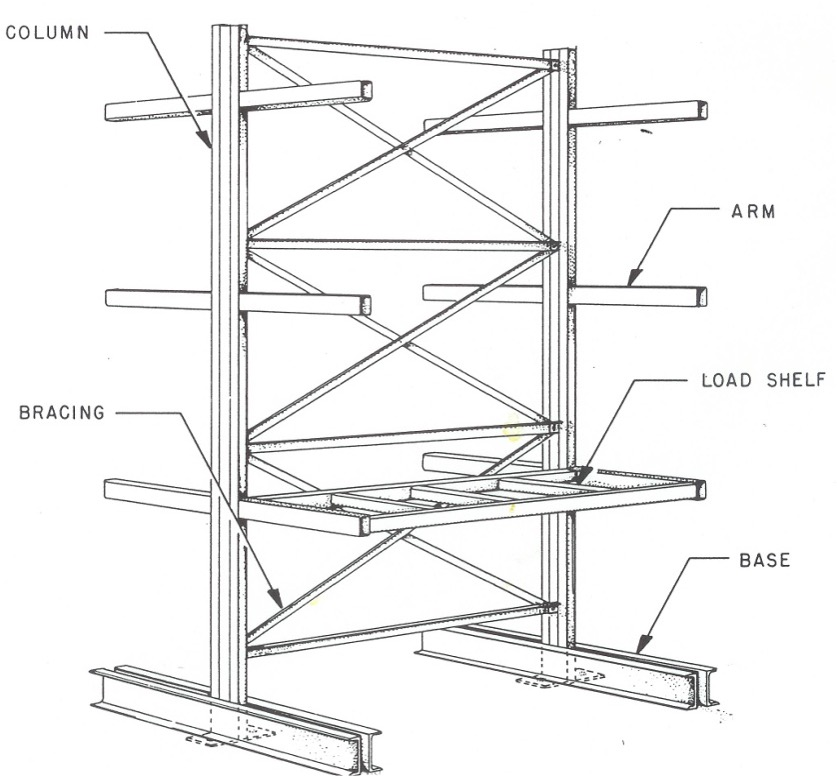
\includegraphics[width=\linewidth]{assets/26.jpg}
        \caption{Cantilever}\label{fig:Cantilever}
    \end{subfigure}
    \begin{subfigure}{0.45\linewidth}
        \centering
        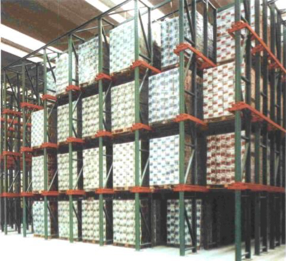
\includegraphics[width=\linewidth]{assets/27.png}
        \caption{Scaffalature Pesanti}\label{fig:peso}
    \end{subfigure}

    \caption{}\label{fig:}
\end{figure}
%
\paragraph{Catasta (Block Stacking)} UdC sovrapposte a terra.
Sono semplici, a basso costo e alto sfruttamento superficiale (se pochi codici).
Hanno però selettività bassa ($ \text{selettività}\leq 1 $), stabilità limitata (max 5-6 livelli), bassa potenzialità di movimentazione.

Vedi figura \ref{fig:catasta}.
%
\paragraph{Scaffalature Tradizionali (Bifronte)} Accessibili da entrambi i lati. Ha selettività massima ($ \text{selettività} = 1 $), nessun vincolo di prelievo. Lo sfruttamento dello spazio diminuisce all'aumentare della larghezza dei corridoi.

Vedi figura \ref{fig:scaffalatura_trad}
%
\paragraph{Cantilever}
Struttura a mensole per carichi lunghi (barre, tubi).

Vedi figura \ref{fig:Cantilever}.

%
\paragraph{Scaffalature Passanti (Drive-in / Drive-through)} Il carrello entra nello scaffale.
\begin{itemize}
    \item \textbf{Drive-in}: Accesso da un solo lato (LIFO - Last In First Out);
    \item \textbf{Drive-through}: Accesso da lati opposti (FIFO - First In First Out);
    \item \textbf{Pro}: Alta densità volumetrica ($ >80\% $). Adatto a bassa varietà di prodotti.
\end{itemize}

Vedi figura \ref{fig:peso}.
%
\subsection{Magazzini Dinamici}
Questi sistemi riducono i corridoi per massimizzare lo spazio.
%
\paragraph{A Gravità (Live Storage)} Rulliere inclinate (3-4\%).
\begin{itemize}
    \item \textbf{Logica}: FIFO.
    \item \textbf{Caratteristiche}: Alto sfruttamento volumetrico, eliminazione corridoi intermedi. Costo elevato.
\end{itemize}
%
\paragraph{Flow Rail} Movimentazione tramite catena dentata sui binari.
\begin{itemize}
    \item \textbf{Logica}: LIFO orizzontale. Stoccaggio fino a 12 pallet in profondità. Alta densità (+40\%).
\end{itemize}

%
\paragraph{Psuh Back} Carrelli su guide telescopiche, spinti dall'inserimento del pallet successivo.
\begin{itemize}
    \item \textbf{Logica}: LIFO. Adatto a carichi uniformi, max 3-4 pallet per canale.
\end{itemize}

%
\paragraph{Magazzini a Satellite (Pallet Shuttle)} Una navetta (satellite) si muove autonomamente nel canale.
\begin{itemize}
    \item \textbf{Vantaggi}: Alta velocità ($ 90 \si{m\per\min} $ scarico), canali profondi (fino a $ 40 \si{\m} $), flessibilità (LIFO o FIFO), aumento cicli/ora.
\end{itemize}

%
\paragraph{Scaffali Mobili (Compattabili)} Scaffali montati su basi mobili che scorrono su binari, aprendo il corridoio solo dove serve.
\begin{itemize}
    \item \textbf{Pro}: Risparmio 50\% superficie, incremento 180\% capacità.
    \item \textbf{Contro}: Bassa velocità di accesso (non adatto ad alta rotazione), costi elevati.
\end{itemize}

%
\section{Calcoli di Dimensionamento}
Guarda la tabella \ref{tab:formule_carrelli} per il riepilogo delle formule.
%
\paragraph{Coefficiente di Utilizzazione Superficiale}
Utilizziamo coem esempio gli scaffali bifronte:
\begin{enumerate}
    \item Calcolare l'area del modulo unitario (es: profondità scaffale + metà corridoio per lato);
    \item Calcolare il numero di pallet per modulo (livelli in altezza);
    \item Rapportare i pallet all'area: $\si{Pallet\per\m^2}$
\end{enumerate}

%
\paragraph{Sistema di Movimentazione}
Durata media dei cicli di prelievo/immissione dipende da:
\begin{itemize}
    \item lay-out delle scaffalature;
    \item allocazione fisica degli articoli;
    \item caratteristica dei cicli (semplici o combinati);
    \item prestazione dei mezzi di movimentazione e relativa modalità operative;
    \item gestione delle operazioni;
    \item punto di accesso.
\end{itemize}
%
\subparagraph{Tempo Ciclo}
Inoltre calcoliamo il tempo ciclo medio che utilizzeremo poi per determinare quanti carrelli ($ z $) sono necessari.
\[
    \text{Tempo Ciclo} = \text{Tempo Fisso} + \text{Tempo Variabile}
\]

%
\subsection{Numero di Carrelli}
\begin{figure}
    \centering
    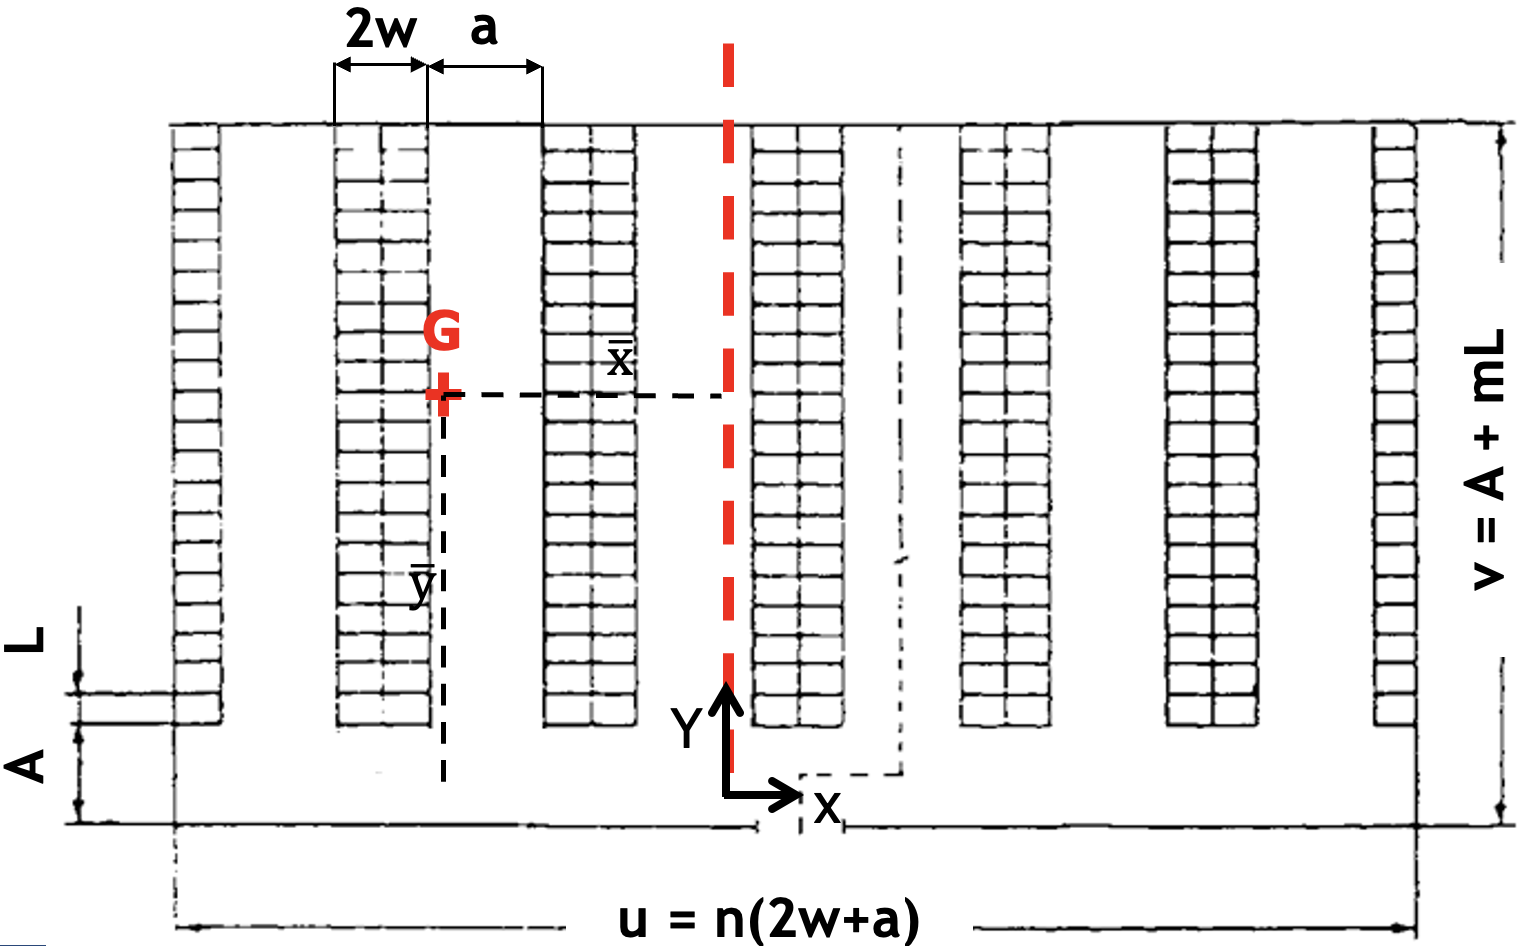
\includegraphics[width=0.7\linewidth]{assets/Screenshot 2026-01-26 at 15.42.52.png}
    \caption{Disposizione scaffalature}\label{fig:disp}
\end{figure}
Si consideri la disposizione delle scaffalature viste in figura \ref{fig:disp}, inoltre si ipotizzi che il nostro magazzino ha:
\begin{itemize}
    \item scaffalature bifrontali;
    \item cicli semplici;
    \item percorsi rettilinei;
    \item equiprobabilità di accesso a qualsiasi vano;
    \item punto di accesso (carico/scarico) al centro del fronte scaffalatura.
\end{itemize}
%
\paragraph{Percorso totale medio} Il percorso totale medio per la movimentazione di unità di carico ($ r $) si determina considerando il viaggio di andata e ritorno:
\begin{gather*}
    r = 2 \cdot 2 \cdot (\overline{x}+\overline{y}) = 2 \cdot 2 \cdot (\frac{n \cdot (2w + a)}{4}+(\frac{m \cdot l}{2}+A)) \\
    \downarrow \\
    r = n \cdot (2w+a)+ 2 \cdot (2A+m \cdot l)
\end{gather*}
Dove:
\begin{itemize}
    \item $n$=corridoi;
    \item $w$=larghezza laterale;
    \item $a$=larghezza corridoio;
    \item $A$=spazio testata;
    \item $m$=numero pallet in lunghezza;
    \item $l$=larghezza posto pallet.
\end{itemize}

%
\paragraph{Durata del ciclo} La durata del ciclo di movimentazione ($ d $) è la somma dei tempi di viaggio, sollevamento e tempi fissi ($ t_{f} $):
\begin{gather*}
    d = \frac{r}{v_{t}}+\frac{2 \cdot 2 \cdot h \cdot (j-1)}{2 \cdot v_{s}} + t_{f} \\
    \downarrow \\
    d = \frac{r}{v_{t}}+\frac{2 \cdot h \cdot (j-1)}{v_{s}} + t_{f}
\end{gather*}
Dove:
\begin{itemize}
    \item $v_t$: Velocità traslazione;
    \item $v_s$: Velocità sollevamento;
    \item $h$: Altezza posto pallet;
    \item $j$: Numero livelli.
    \item $ t_{f} $: Somma dei tempi fissi (immissione + prelievo)
\end{itemize}

%
\paragraph{Numero di carrelli}
Il numero di carrelli ($ z $) si calcola con:
\[
    z = \frac{d \cdot f}{g \cdot y \cdot \eta}
\]
Dove:
\begin{itemize}
    \item $ f $: Pallet movimentati in un anno (o altro periodo di tempo di riferimento);
    \item $ g $: Ore di funzionamento al giorno;
    \item $ y $: Giorni in un anno;
    \item $ \eta $ (eta): Coefficiente di utilizzazione.
\end{itemize}
\begin{table}
    \centering
    \renewcommand{\arraystretch}{2.0} % Aumenta lo spazio per le frazioni e le formule
    \begin{tabular}{ll} % Due colonne: Nome a sinistra, Formula al centro
        \toprule
        \textbf{Descrizione}        & \textbf{Formula}                                                   \\
        \midrule
        Tempo Ciclo                 & $\text{Tempo Ciclo} = \text{Tempo Fisso} + \text{Tempo Variabile}$ \\
        Percorso totale medio ($r$) & $r = n \cdot (2w+a)+ 2 \cdot (2A+m \cdot l)$                       \\
        Durata del ciclo ($d$)      & $d = \frac{r}{v_{t}}+\frac{2 \cdot h \cdot (j-1)}{v_{s}} + t_{f}$  \\
        Numero di carrelli ($z$)    & $z = \frac{d \cdot f}{g \cdot y \cdot \eta}$                       \\
        \bottomrule
    \end{tabular}
    \caption{Formule per il dimensionamento del sistema di movimentazione}\label{tab:formule_carrelli}
\end{table}
%
\section{e-Commerce}
La progettazione per l'e-commerce richiede estrema flessibilità e gestione di ordini frammentati. Soluzioni tipiche includono scaffalature multilivello (bassi livelli per alta rotazione/picking, alti per riserva) e sistemi compattabili per massimizzare lo spazio.